\documentclass[1p]{elsarticle_modified}
%\bibliographystyle{elsarticle-num}

%\usepackage[colorlinks]{hyperref}
%\usepackage{abbrmath_seonhwa} %\Abb, \Ascr, \Acal ,\Abf, \Afrak
\usepackage{amsfonts}
\usepackage{amssymb}
\usepackage{amsmath}
\usepackage{amsthm}
\usepackage{scalefnt}
\usepackage{amsbsy}
\usepackage{kotex}
\usepackage{caption}
\usepackage{subfig}
\usepackage{color}
\usepackage{graphicx}
\usepackage{xcolor} %% white, black, red, green, blue, cyan, magenta, yellow
\usepackage{float}
\usepackage{setspace}
\usepackage{hyperref}

\usepackage{tikz}
\usetikzlibrary{arrows}

\usepackage{multirow}
\usepackage{array} % fixed length table
\usepackage{hhline}

%%%%%%%%%%%%%%%%%%%%%
\makeatletter
\renewcommand*\env@matrix[1][\arraystretch]{%
	\edef\arraystretch{#1}%
	\hskip -\arraycolsep
	\let\@ifnextchar\new@ifnextchar
	\array{*\c@MaxMatrixCols c}}
\makeatother %https://tex.stackexchange.com/questions/14071/how-can-i-increase-the-line-spacing-in-a-matrix
%%%%%%%%%%%%%%%

\usepackage[normalem]{ulem}

\newcommand{\msout}[1]{\ifmmode\text{\sout{\ensuremath{#1}}}\else\sout{#1}\fi}
%SOURCE: \msout is \stkout macro in https://tex.stackexchange.com/questions/20609/strikeout-in-math-mode

\newcommand{\cancel}[1]{
	\ifmmode
	{\color{red}\msout{#1}}
	\else
	{\color{red}\sout{#1}}
	\fi
}

\newcommand{\add}[1]{
	{\color{blue}\uwave{#1}}
}

\newcommand{\replace}[2]{
	\ifmmode
	{\color{red}\msout{#1}}{\color{blue}\uwave{#2}}
	\else
	{\color{red}\sout{#1}}{\color{blue}\uwave{#2}}
	\fi
}

\newcommand{\Sol}{\mathcal{S}} %segment
\newcommand{\D}{D} %diagram
\newcommand{\A}{\mathcal{A}} %arc


%%%%%%%%%%%%%%%%%%%%%%%%%%%%%5 test

\def\sl{\operatorname{\textup{SL}}(2,\Cbb)}
\def\psl{\operatorname{\textup{PSL}}(2,\Cbb)}
\def\quan{\mkern 1mu \triangleright \mkern 1mu}

\theoremstyle{definition}
\newtheorem{thm}{Theorem}[section]
\newtheorem{prop}[thm]{Proposition}
\newtheorem{lem}[thm]{Lemma}
\newtheorem{ques}[thm]{Question}
\newtheorem{cor}[thm]{Corollary}
\newtheorem{defn}[thm]{Definition}
\newtheorem{exam}[thm]{Example}
\newtheorem{rmk}[thm]{Remark}
\newtheorem{alg}[thm]{Algorithm}

\newcommand{\I}{\sqrt{-1}}
\begin{document}

%\begin{frontmatter}
%
%\title{Boundary parabolic representations of knots up to 8 crossings}
%
%%% Group authors per affiliation:
%\author{Yunhi Cho} 
%\address{Department of Mathematics, University of Seoul, Seoul, Korea}
%\ead{yhcho@uos.ac.kr}
%
%
%\author{Seonhwa Kim} %\fnref{s_kim}}
%\address{Center for Geometry and Physics, Institute for Basic Science, Pohang, 37673, Korea}
%\ead{ryeona17@ibs.re.kr}
%
%\author{Hyuk Kim}
%\address{Department of Mathematical Sciences, Seoul National University, Seoul 08826, Korea}
%\ead{hyukkim@snu.ac.kr}
%
%\author{Seokbeom Yoon}
%\address{Department of Mathematical Sciences, Seoul National University, Seoul, 08826,  Korea}
%\ead{sbyoon15@snu.ac.kr}
%
%\begin{abstract}
%We find all boundary parabolic representation of knots up to 8 crossings.
%
%\end{abstract}
%\begin{keyword}
%    \MSC[2010] 57M25 
%\end{keyword}
%
%\end{frontmatter}

%\linenumbers
%\tableofcontents
%
\newcommand\colored[1]{\textcolor{white}{\rule[-0.35ex]{0.8em}{1.4ex}}\kern-0.8em\color{red} #1}%
%\newcommand\colored[1]{\textcolor{white}{ #1}\kern-2.17ex	\textcolor{white}{ #1}\kern-1.81ex	\textcolor{white}{ #1}\kern-2.15ex\color{red}#1	}

{\Large $\underline{12a_{0573}~(K12a_{0573})}$}

\setlength{\tabcolsep}{10pt}
\renewcommand{\arraystretch}{1.6}
\vspace{1cm}\begin{tabular}{m{100pt}>{\centering\arraybackslash}m{274pt}}
\multirow{5}{120pt}{
	\centering
	\includegraphics[width=112pt]{../../../GIT/diagram.site/Diagrams/png/1374_12a_0573.png}\\
\ \ \ A knot diagram\footnotemark}&
\allowdisplaybreaks
\textbf{Linearized knot diagam} \\
\cline{2-2}
 &
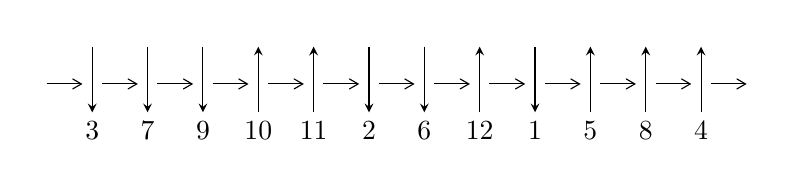
\begin{tikzpicture}[x=20pt, y=17pt]
	% nodes
	\node (C0) at (0, 0) {};
	\node (C1) at (1, 0) {};
	\node (C1U) at (1, +1) {};
	\node (C1D) at (1, -1) {3};

	\node (C2) at (2, 0) {};
	\node (C2U) at (2, +1) {};
	\node (C2D) at (2, -1) {7};

	\node (C3) at (3, 0) {};
	\node (C3U) at (3, +1) {};
	\node (C3D) at (3, -1) {9};

	\node (C4) at (4, 0) {};
	\node (C4U) at (4, +1) {};
	\node (C4D) at (4, -1) {10};

	\node (C5) at (5, 0) {};
	\node (C5U) at (5, +1) {};
	\node (C5D) at (5, -1) {11};

	\node (C6) at (6, 0) {};
	\node (C6U) at (6, +1) {};
	\node (C6D) at (6, -1) {2};

	\node (C7) at (7, 0) {};
	\node (C7U) at (7, +1) {};
	\node (C7D) at (7, -1) {6};

	\node (C8) at (8, 0) {};
	\node (C8U) at (8, +1) {};
	\node (C8D) at (8, -1) {12};

	\node (C9) at (9, 0) {};
	\node (C9U) at (9, +1) {};
	\node (C9D) at (9, -1) {1};

	\node (C10) at (10, 0) {};
	\node (C10U) at (10, +1) {};
	\node (C10D) at (10, -1) {5};

	\node (C11) at (11, 0) {};
	\node (C11U) at (11, +1) {};
	\node (C11D) at (11, -1) {8};

	\node (C12) at (12, 0) {};
	\node (C12U) at (12, +1) {};
	\node (C12D) at (12, -1) {4};
	\node (C13) at (13, 0) {};

	% arrows
	\draw[->,>={angle 60}]
	(C0) edge (C1) (C1) edge (C2) (C2) edge (C3) (C3) edge (C4) (C4) edge (C5) (C5) edge (C6) (C6) edge (C7) (C7) edge (C8) (C8) edge (C9) (C9) edge (C10) (C10) edge (C11) (C11) edge (C12) (C12) edge (C13) ;	\draw[->,>=stealth]
	(C1U) edge (C1D) (C2U) edge (C2D) (C3U) edge (C3D) (C4D) edge (C4U) (C5D) edge (C5U) (C6U) edge (C6D) (C7U) edge (C7D) (C8D) edge (C8U) (C9U) edge (C9D) (C10D) edge (C10U) (C11D) edge (C11U) (C12D) edge (C12U) ;
	\end{tikzpicture} \\
\hhline{~~} \\& 
\textbf{Solving Sequence} \\ \cline{2-2} 
 &
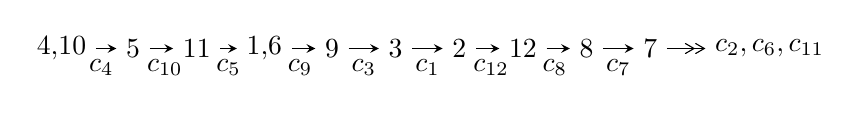
\begin{tikzpicture}[x=23pt, y=7pt]
	% node
	\node (A0) at (-1/8, 0) {4,10};
	\node (A1) at (1, 0) {5};
	\node (A2) at (2, 0) {11};
	\node (A3) at (49/16, 0) {1,6};
	\node (A4) at (33/8, 0) {9};
	\node (A5) at (41/8, 0) {3};
	\node (A6) at (49/8, 0) {2};
	\node (A7) at (57/8, 0) {12};
	\node (A8) at (65/8, 0) {8};
	\node (A9) at (73/8, 0) {7};
	\node (C1) at (1/2, -1) {$c_{4}$};
	\node (C2) at (3/2, -1) {$c_{10}$};
	\node (C3) at (5/2, -1) {$c_{5}$};
	\node (C4) at (29/8, -1) {$c_{9}$};
	\node (C5) at (37/8, -1) {$c_{3}$};
	\node (C6) at (45/8, -1) {$c_{1}$};
	\node (C7) at (53/8, -1) {$c_{12}$};
	\node (C8) at (61/8, -1) {$c_{8}$};
	\node (C9) at (69/8, -1) {$c_{7}$};
	\node (A10) at (11, 0) {$c_{2},c_{6},c_{11}$};

	% edge
	\draw[->,>=stealth]	
	(A0) edge (A1) (A1) edge (A2) (A2) edge (A3) (A3) edge (A4) (A4) edge (A5) (A5) edge (A6) (A6) edge (A7) (A7) edge (A8) (A8) edge (A9) ;
	\draw[->>,>={angle 60}]	
	(A9) edge (A10);
\end{tikzpicture} \\ 

\end{tabular} \\

\footnotetext{
The image of knot diagram is generated by the software ``\textbf{Draw programme}" developed by Andrew Bartholomew(\url{http://www.layer8.co.uk/maths/draw/index.htm\#Running-draw}), where we modified some parts for our purpose(\url{https://github.com/CATsTAILs/LinksPainter}).
}\phantom \\ \newline 
\centering \textbf{Ideals for irreducible components\footnotemark of $X_{\text{par}}$} 
 
\begin{align*}
I^u_{1}&=\langle 
7.55432\times10^{231} u^{94}-3.94979\times10^{231} u^{93}+\cdots+5.03123\times10^{233} b+8.02484\times10^{234},\\
\phantom{I^u_{1}}&\phantom{= \langle  }-6.27990\times10^{234} u^{94}+4.91845\times10^{234} u^{93}+\cdots+3.84051\times10^{235} a-5.98614\times10^{237},\\
\phantom{I^u_{1}}&\phantom{= \langle  }u^{95}- u^{94}+\cdots+998 u-229\rangle \\
I^u_{2}&=\langle 
- u^{21}+12 u^{19}+\cdots+b+1,\;- u^{23}+13 u^{21}+\cdots+a+u,\;u^{24}-14 u^{22}+\cdots+2 u-1\rangle \\
\\
\end{align*}
\raggedright * 2 irreducible components of $\dim_{\mathbb{C}}=0$, with total 119 representations.\\
\footnotetext{All coefficients of polynomials are rational numbers. But the coefficients are sometimes approximated in decimal forms when there is not enough margin.}
\newpage
\renewcommand{\arraystretch}{1}
\centering \section*{I. $I^u_{1}= \langle 7.55\times10^{231} u^{94}-3.95\times10^{231} u^{93}+\cdots+5.03\times10^{233} b+8.02\times10^{234},\;-6.28\times10^{234} u^{94}+4.92\times10^{234} u^{93}+\cdots+3.84\times10^{235} a-5.99\times10^{237},\;u^{95}- u^{94}+\cdots+998 u-229 \rangle$}
\flushleft \textbf{(i) Arc colorings}\\
\begin{tabular}{m{7pt} m{180pt} m{7pt} m{180pt} }
\flushright $a_{4}=$&$\begin{pmatrix}1\\0\end{pmatrix}$ \\
\flushright $a_{10}=$&$\begin{pmatrix}0\\u\end{pmatrix}$ \\
\flushright $a_{5}=$&$\begin{pmatrix}1\\- u^2\end{pmatrix}$ \\
\flushright $a_{11}=$&$\begin{pmatrix}u\\- u^3+u\end{pmatrix}$ \\
\flushright $a_{1}=$&$\begin{pmatrix}0.163517 u^{94}-0.128068 u^{93}+\cdots-9.60245 u+155.869\\-0.0150148 u^{94}+0.00785054 u^{93}+\cdots+7.03716 u-15.9501\end{pmatrix}$ \\
\flushright $a_{6}=$&$\begin{pmatrix}- u^2+1\\u^4-2 u^2\end{pmatrix}$ \\
\flushright $a_{9}=$&$\begin{pmatrix}0.149130 u^{94}-0.101058 u^{93}+\cdots-50.2226 u+125.337\\-0.0388424 u^{94}+0.0317280 u^{93}+\cdots+9.44989 u-34.1884\end{pmatrix}$ \\
\flushright $a_{3}=$&$\begin{pmatrix}-0.199431 u^{94}+0.152151 u^{93}+\cdots+59.9789 u-181.897\\0.0125942 u^{94}-0.0169786 u^{93}+\cdots+12.7547 u+21.1136\end{pmatrix}$ \\
\flushright $a_{2}=$&$\begin{pmatrix}0.242375 u^{94}-0.182145 u^{93}+\cdots-44.1731 u+223.500\\-0.00939841 u^{94}+0.00780443 u^{93}+\cdots-6.28912 u-14.2852\end{pmatrix}$ \\
\flushright $a_{12}=$&$\begin{pmatrix}0.178532 u^{94}-0.135918 u^{93}+\cdots-16.6396 u+171.819\\-0.0150148 u^{94}+0.00785054 u^{93}+\cdots+7.03716 u-15.9501\end{pmatrix}$ \\
\flushright $a_{8}=$&$\begin{pmatrix}-0.0921952 u^{94}+0.0767583 u^{93}+\cdots+13.7278 u-100.851\\-4.09274\times10^{-6} u^{94}+0.00284681 u^{93}+\cdots+4.30488 u-3.91892\end{pmatrix}$ \\
\flushright $a_{7}=$&$\begin{pmatrix}-0.0978961 u^{94}+0.0863550 u^{93}+\cdots+12.3830 u-113.021\\-0.00892542 u^{94}+0.0100792 u^{93}+\cdots+13.6694 u-5.66045\end{pmatrix}$\\&\end{tabular}
\flushleft \textbf{(ii) Obstruction class $= -1$}\\~\\
\flushleft \textbf{(iii) Cusp Shapes $= -0.418076 u^{94}+0.342082 u^{93}+\cdots-2.01058 u-379.553$}\\~\\
\newpage\renewcommand{\arraystretch}{1}
\flushleft \textbf{(iv) u-Polynomials at the component}\newline \\
\begin{tabular}{m{50pt}|m{274pt}}
Crossings & \hspace{64pt}u-Polynomials at each crossing \\
\hline $$\begin{aligned}c_{1},c_{7}\end{aligned}$$&$\begin{aligned}
&u^{95}+27 u^{94}+\cdots+25 u+1
\end{aligned}$\\
\hline $$\begin{aligned}c_{2},c_{6}\end{aligned}$$&$\begin{aligned}
&u^{95}- u^{94}+\cdots+u+1
\end{aligned}$\\
\hline $$\begin{aligned}c_{3}\end{aligned}$$&$\begin{aligned}
&u^{95}- u^{94}+\cdots-3835 u+845
\end{aligned}$\\
\hline $$\begin{aligned}c_{4},c_{5},c_{10}\end{aligned}$$&$\begin{aligned}
&u^{95}+u^{94}+\cdots+998 u+229
\end{aligned}$\\
\hline $$\begin{aligned}c_{8},c_{11}\end{aligned}$$&$\begin{aligned}
&u^{95}+u^{94}+\cdots-18 u+1
\end{aligned}$\\
\hline $$\begin{aligned}c_{9}\end{aligned}$$&$\begin{aligned}
&u^{95}+7 u^{94}+\cdots-15768 u+1413
\end{aligned}$\\
\hline $$\begin{aligned}c_{12}\end{aligned}$$&$\begin{aligned}
&u^{95}+8 u^{94}+\cdots+17711 u+2447
\end{aligned}$\\
\hline
\end{tabular}\\~\\
\newpage\renewcommand{\arraystretch}{1}
\flushleft \textbf{(v) Riley Polynomials at the component}\newline \\
\begin{tabular}{m{50pt}|m{274pt}}
Crossings & \hspace{64pt}Riley Polynomials at each crossing \\
\hline $$\begin{aligned}c_{1},c_{7}\end{aligned}$$&$\begin{aligned}
&y^{95}+93 y^{94}+\cdots+225 y-1
\end{aligned}$\\
\hline $$\begin{aligned}c_{2},c_{6}\end{aligned}$$&$\begin{aligned}
&y^{95}-27 y^{94}+\cdots+25 y-1
\end{aligned}$\\
\hline $$\begin{aligned}c_{3}\end{aligned}$$&$\begin{aligned}
&y^{95}+31 y^{94}+\cdots-12307425 y-714025
\end{aligned}$\\
\hline $$\begin{aligned}c_{4},c_{5},c_{10}\end{aligned}$$&$\begin{aligned}
&y^{95}-109 y^{94}+\cdots+3539736 y-52441
\end{aligned}$\\
\hline $$\begin{aligned}c_{8},c_{11}\end{aligned}$$&$\begin{aligned}
&y^{95}-93 y^{94}+\cdots+92 y-1
\end{aligned}$\\
\hline $$\begin{aligned}c_{9}\end{aligned}$$&$\begin{aligned}
&y^{95}+35 y^{94}+\cdots+42933762 y-1996569
\end{aligned}$\\
\hline $$\begin{aligned}c_{12}\end{aligned}$$&$\begin{aligned}
&y^{95}-36 y^{94}+\cdots+298346619 y-5987809
\end{aligned}$\\
\hline
\end{tabular}\\~\\
\newpage\flushleft \textbf{(vi) Complex Volumes and Cusp Shapes}
$$\begin{array}{c|c|c}  
\text{Solutions to }I^u_{1}& \I (\text{vol} + \sqrt{-1}CS) & \text{Cusp shape}\\
 \hline 
\begin{aligned}
u &= -0.993324 + 0.113886 I \\
a &= -0.211155 - 0.035291 I \\
b &= \phantom{-}0.474145 + 0.672640 I\end{aligned}
 & \phantom{-}1.75972 - 0.04833 I & \phantom{-0.000000 } 0 \\ \hline\begin{aligned}
u &= -0.993324 - 0.113886 I \\
a &= -0.211155 + 0.035291 I \\
b &= \phantom{-}0.474145 - 0.672640 I\end{aligned}
 & \phantom{-}1.75972 + 0.04833 I & \phantom{-0.000000 } 0 \\ \hline\begin{aligned}
u &= \phantom{-}0.996175 + 0.200215 I \\
a &= \phantom{-}0.444838 - 0.245934 I \\
b &= \phantom{-}0.027663 - 0.803448 I\end{aligned}
 & \phantom{-}1.26759 + 4.32682 I & \phantom{-0.000000 } 0 \\ \hline\begin{aligned}
u &= \phantom{-}0.996175 - 0.200215 I \\
a &= \phantom{-}0.444838 + 0.245934 I \\
b &= \phantom{-}0.027663 + 0.803448 I\end{aligned}
 & \phantom{-}1.26759 - 4.32682 I & \phantom{-0.000000 } 0 \\ \hline\begin{aligned}
u &= -0.696166 + 0.748256 I \\
a &= \phantom{-}0.582098 - 0.191531 I \\
b &= \phantom{-}0.767229 + 0.497403 I\end{aligned}
 & \phantom{-}1.18820 + 2.86171 I & \phantom{-0.000000 } 0 \\ \hline\begin{aligned}
u &= -0.696166 - 0.748256 I \\
a &= \phantom{-}0.582098 + 0.191531 I \\
b &= \phantom{-}0.767229 - 0.497403 I\end{aligned}
 & \phantom{-}1.18820 - 2.86171 I & \phantom{-0.000000 } 0 \\ \hline\begin{aligned}
u &= -0.535987 + 0.636878 I \\
a &= \phantom{-}0.234758 - 1.306110 I \\
b &= \phantom{-}1.134930 - 0.783701 I\end{aligned}
 & \phantom{-}0.91102 - 7.57603 I & \phantom{-0.000000 } 0 \\ \hline\begin{aligned}
u &= -0.535987 - 0.636878 I \\
a &= \phantom{-}0.234758 + 1.306110 I \\
b &= \phantom{-}1.134930 + 0.783701 I\end{aligned}
 & \phantom{-}0.91102 + 7.57603 I & \phantom{-0.000000 } 0 \\ \hline\begin{aligned}
u &= \phantom{-}0.731945 + 0.345316 I \\
a &= \phantom{-}0.008581 - 1.276130 I \\
b &= -1.14528 - 0.86552 I\end{aligned}
 & \phantom{-}3.71584 + 3.90274 I & \phantom{-0.000000 } 0 \\ \hline\begin{aligned}
u &= \phantom{-}0.731945 - 0.345316 I \\
a &= \phantom{-}0.008581 + 1.276130 I \\
b &= -1.14528 + 0.86552 I\end{aligned}
 & \phantom{-}3.71584 - 3.90274 I & \phantom{-0.000000 } 0\\
 \hline 
 \end{array}$$\newpage$$\begin{array}{c|c|c}  
\text{Solutions to }I^u_{1}& \I (\text{vol} + \sqrt{-1}CS) & \text{Cusp shape}\\
 \hline 
\begin{aligned}
u &= \phantom{-}0.225383 + 0.749670 I \\
a &= -1.118140 - 0.145739 I \\
b &= -0.758397 + 0.405896 I\end{aligned}
 & \phantom{-}1.56332 - 0.38085 I & \phantom{-0.000000 } 0 \\ \hline\begin{aligned}
u &= \phantom{-}0.225383 - 0.749670 I \\
a &= -1.118140 + 0.145739 I \\
b &= -0.758397 - 0.405896 I\end{aligned}
 & \phantom{-}1.56332 + 0.38085 I & \phantom{-0.000000 } 0 \\ \hline\begin{aligned}
u &= -0.777312 + 0.950438 I \\
a &= \phantom{-}0.270161 - 1.108820 I \\
b &= \phantom{-}1.087020 - 0.803080 I\end{aligned}
 & \phantom{-}8.6020 - 12.0514 I & \phantom{-0.000000 } 0 \\ \hline\begin{aligned}
u &= -0.777312 - 0.950438 I \\
a &= \phantom{-}0.270161 + 1.108820 I \\
b &= \phantom{-}1.087020 + 0.803080 I\end{aligned}
 & \phantom{-}8.6020 + 12.0514 I & \phantom{-0.000000 } 0 \\ \hline\begin{aligned}
u &= \phantom{-}0.840314 + 0.900458 I \\
a &= -0.241403 - 1.100060 I \\
b &= -1.089160 - 0.808193 I\end{aligned}
 & \phantom{-}9.11645 + 5.73244 I & \phantom{-0.000000 } 0 \\ \hline\begin{aligned}
u &= \phantom{-}0.840314 - 0.900458 I \\
a &= -0.241403 + 1.100060 I \\
b &= -1.089160 + 0.808193 I\end{aligned}
 & \phantom{-}9.11645 - 5.73244 I & \phantom{-0.000000 } 0 \\ \hline\begin{aligned}
u &= -0.757972 + 0.007541 I \\
a &= -0.829238 + 0.252949 I \\
b &= \phantom{-}0.532454 - 0.236617 I\end{aligned}
 & \phantom{-}1.67673 - 0.14877 I & \phantom{-0.000000 } 0 \\ \hline\begin{aligned}
u &= -0.757972 - 0.007541 I \\
a &= -0.829238 - 0.252949 I \\
b &= \phantom{-}0.532454 + 0.236617 I\end{aligned}
 & \phantom{-}1.67673 + 0.14877 I & \phantom{-0.000000 } 0 \\ \hline\begin{aligned}
u &= \phantom{-}0.623797 + 0.414333 I \\
a &= \phantom{-}0.228053 + 1.275920 I \\
b &= -0.95365 + 1.12669 I\end{aligned}
 & \phantom{-}8.09696 - 1.35610 I & \phantom{-0.000000 } 0 \\ \hline\begin{aligned}
u &= \phantom{-}0.623797 - 0.414333 I \\
a &= \phantom{-}0.228053 - 1.275920 I \\
b &= -0.95365 - 1.12669 I\end{aligned}
 & \phantom{-}8.09696 + 1.35610 I & \phantom{-0.000000 } 0\\
 \hline 
 \end{array}$$\newpage$$\begin{array}{c|c|c}  
\text{Solutions to }I^u_{1}& \I (\text{vol} + \sqrt{-1}CS) & \text{Cusp shape}\\
 \hline 
\begin{aligned}
u &= -0.527293 + 0.500564 I \\
a &= -0.206299 + 1.273140 I \\
b &= \phantom{-}0.89031 + 1.16063 I\end{aligned}
 & \phantom{-}7.47429 - 5.04540 I & \phantom{-0.000000 } 0 \\ \hline\begin{aligned}
u &= -0.527293 - 0.500564 I \\
a &= -0.206299 - 1.273140 I \\
b &= \phantom{-}0.89031 - 1.16063 I\end{aligned}
 & \phantom{-}7.47429 + 5.04540 I & \phantom{-0.000000 } 0 \\ \hline\begin{aligned}
u &= -0.549773 + 0.459183 I \\
a &= -2.27573 - 0.21620 I \\
b &= \phantom{-}0.733117 - 0.391883 I\end{aligned}
 & \phantom{-}7.54560 + 1.65750 I & \phantom{-}8.73859 + 0. I\phantom{ +0.000000I} \\ \hline\begin{aligned}
u &= -0.549773 - 0.459183 I \\
a &= -2.27573 + 0.21620 I \\
b &= \phantom{-}0.733117 + 0.391883 I\end{aligned}
 & \phantom{-}7.54560 - 1.65750 I & \phantom{-}8.73859 + 0. I\phantom{ +0.000000I} \\ \hline\begin{aligned}
u &= -0.526692 + 0.472816 I \\
a &= -1.214460 + 0.533716 I \\
b &= -0.693000 + 0.127743 I\end{aligned}
 & \phantom{-}3.39672 - 0.91258 I & \phantom{-0.000000 -}0. + 5.79505 I \\ \hline\begin{aligned}
u &= -0.526692 - 0.472816 I \\
a &= -1.214460 - 0.533716 I \\
b &= -0.693000 - 0.127743 I\end{aligned}
 & \phantom{-}3.39672 + 0.91258 I & \phantom{-0.000000 } 0. - 5.79505 I \\ \hline\begin{aligned}
u &= \phantom{-}0.485680 + 1.199540 I \\
a &= -0.768169 + 0.079709 I \\
b &= -0.843819 + 0.441106 I\end{aligned}
 & \phantom{-}7.84874 + 1.09621 I & \phantom{-0.000000 } 0 \\ \hline\begin{aligned}
u &= \phantom{-}0.485680 - 1.199540 I \\
a &= -0.768169 - 0.079709 I \\
b &= -0.843819 - 0.441106 I\end{aligned}
 & \phantom{-}7.84874 - 1.09621 I & \phantom{-0.000000 } 0 \\ \hline\begin{aligned}
u &= \phantom{-}0.586251 + 0.391592 I \\
a &= -0.06845 + 2.24487 I \\
b &= \phantom{-}0.797329 + 0.528318 I\end{aligned}
 & \phantom{-}2.92370 + 7.46960 I & \phantom{-0.000000 } 0. - 9.77082 I \\ \hline\begin{aligned}
u &= \phantom{-}0.586251 - 0.391592 I \\
a &= -0.06845 - 2.24487 I \\
b &= \phantom{-}0.797329 - 0.528318 I\end{aligned}
 & \phantom{-}2.92370 - 7.46960 I & \phantom{-0.000000 -}0. + 9.77082 I\\
 \hline 
 \end{array}$$\newpage$$\begin{array}{c|c|c}  
\text{Solutions to }I^u_{1}& \I (\text{vol} + \sqrt{-1}CS) & \text{Cusp shape}\\
 \hline 
\begin{aligned}
u &= \phantom{-}0.569131 + 0.398506 I \\
a &= \phantom{-}1.329510 + 0.475836 I \\
b &= \phantom{-}0.707955 + 0.063430 I\end{aligned}
 & \phantom{-}2.74972 - 4.66676 I & \phantom{-0.000000 } 0 \\ \hline\begin{aligned}
u &= \phantom{-}0.569131 - 0.398506 I \\
a &= \phantom{-}1.329510 - 0.475836 I \\
b &= \phantom{-}0.707955 - 0.063430 I\end{aligned}
 & \phantom{-}2.74972 + 4.66676 I & \phantom{-0.000000 } 0 \\ \hline\begin{aligned}
u &= -0.569144 + 1.190100 I \\
a &= \phantom{-}0.732157 + 0.070791 I \\
b &= \phantom{-}0.845166 + 0.455105 I\end{aligned}
 & \phantom{-}7.77827 + 5.11561 I & \phantom{-0.000000 } 0 \\ \hline\begin{aligned}
u &= -0.569144 - 1.190100 I \\
a &= \phantom{-}0.732157 - 0.070791 I \\
b &= \phantom{-}0.845166 - 0.455105 I\end{aligned}
 & \phantom{-}7.77827 - 5.11561 I & \phantom{-0.000000 } 0 \\ \hline\begin{aligned}
u &= \phantom{-}1.317630 + 0.080427 I \\
a &= \phantom{-}0.367515 - 1.052560 I \\
b &= -1.004110 - 0.841707 I\end{aligned}
 & \phantom{-}4.85394 + 3.18451 I & \phantom{-0.000000 } 0 \\ \hline\begin{aligned}
u &= \phantom{-}1.317630 - 0.080427 I \\
a &= \phantom{-}0.367515 + 1.052560 I \\
b &= -1.004110 + 0.841707 I\end{aligned}
 & \phantom{-}4.85394 - 3.18451 I & \phantom{-0.000000 } 0 \\ \hline\begin{aligned}
u &= \phantom{-}1.314690 + 0.245234 I \\
a &= \phantom{-}0.194689 - 0.877843 I \\
b &= -1.060160 - 0.841163 I\end{aligned}
 & \phantom{-}4.92156 + 3.67064 I & \phantom{-0.000000 } 0 \\ \hline\begin{aligned}
u &= \phantom{-}1.314690 - 0.245234 I \\
a &= \phantom{-}0.194689 + 0.877843 I \\
b &= -1.060160 + 0.841163 I\end{aligned}
 & \phantom{-}4.92156 - 3.67064 I & \phantom{-0.000000 } 0 \\ \hline\begin{aligned}
u &= \phantom{-}0.355208 + 0.557436 I \\
a &= \phantom{-}0.29330 + 1.68999 I \\
b &= \phantom{-}0.660249 + 0.621988 I\end{aligned}
 & -2.52906 + 3.25489 I & -5.36852 - 7.70712 I \\ \hline\begin{aligned}
u &= \phantom{-}0.355208 - 0.557436 I \\
a &= \phantom{-}0.29330 - 1.68999 I \\
b &= \phantom{-}0.660249 - 0.621988 I\end{aligned}
 & -2.52906 - 3.25489 I & -5.36852 + 7.70712 I\\
 \hline 
 \end{array}$$\newpage$$\begin{array}{c|c|c}  
\text{Solutions to }I^u_{1}& \I (\text{vol} + \sqrt{-1}CS) & \text{Cusp shape}\\
 \hline 
\begin{aligned}
u &= -1.341290 + 0.156139 I \\
a &= -0.409309 - 0.555943 I \\
b &= \phantom{-}1.19066 - 0.80574 I\end{aligned}
 & \phantom{-}2.86230 - 0.93905 I & \phantom{-0.000000 } 0 \\ \hline\begin{aligned}
u &= -1.341290 - 0.156139 I \\
a &= -0.409309 + 0.555943 I \\
b &= \phantom{-}1.19066 + 0.80574 I\end{aligned}
 & \phantom{-}2.86230 + 0.93905 I & \phantom{-0.000000 } 0 \\ \hline\begin{aligned}
u &= \phantom{-}0.461528 + 0.457013 I \\
a &= \phantom{-}2.56177 - 0.19449 I \\
b &= -0.721443 - 0.392720 I\end{aligned}
 & \phantom{-}7.56513 + 4.46649 I & \phantom{-}8.81708 - 7.74250 I \\ \hline\begin{aligned}
u &= \phantom{-}0.461528 - 0.457013 I \\
a &= \phantom{-}2.56177 + 0.19449 I \\
b &= -0.721443 + 0.392720 I\end{aligned}
 & \phantom{-}7.56513 - 4.46649 I & \phantom{-}8.81708 + 7.74250 I \\ \hline\begin{aligned}
u &= \phantom{-}0.580018 + 0.245313 I \\
a &= \phantom{-}0.910584 - 0.070935 I \\
b &= \phantom{-}0.410463 - 0.198520 I\end{aligned}
 & -1.77575 - 0.09596 I & -5.41324 - 1.06240 I \\ \hline\begin{aligned}
u &= \phantom{-}0.580018 - 0.245313 I \\
a &= \phantom{-}0.910584 + 0.070935 I \\
b &= \phantom{-}0.410463 + 0.198520 I\end{aligned}
 & -1.77575 + 0.09596 I & -5.41324 + 1.06240 I \\ \hline\begin{aligned}
u &= -0.526602 + 0.306350 I \\
a &= -0.04969 + 2.53351 I \\
b &= -0.772656 + 0.489239 I\end{aligned}
 & \phantom{-}3.42392 - 1.76238 I & \phantom{-}3.82353 + 4.55359 I \\ \hline\begin{aligned}
u &= -0.526602 - 0.306350 I \\
a &= -0.04969 - 2.53351 I \\
b &= -0.772656 - 0.489239 I\end{aligned}
 & \phantom{-}3.42392 + 1.76238 I & \phantom{-}3.82353 - 4.55359 I \\ \hline\begin{aligned}
u &= \phantom{-}0.079977 + 0.559249 I \\
a &= \phantom{-}0.133715 + 1.223310 I \\
b &= \phantom{-}0.377541 + 0.807990 I\end{aligned}
 & -1.49124 - 1.49233 I & -5.62608 + 3.32257 I \\ \hline\begin{aligned}
u &= \phantom{-}0.079977 - 0.559249 I \\
a &= \phantom{-}0.133715 - 1.223310 I \\
b &= \phantom{-}0.377541 - 0.807990 I\end{aligned}
 & -1.49124 + 1.49233 I & -5.62608 - 3.32257 I\\
 \hline 
 \end{array}$$\newpage$$\begin{array}{c|c|c}  
\text{Solutions to }I^u_{1}& \I (\text{vol} + \sqrt{-1}CS) & \text{Cusp shape}\\
 \hline 
\begin{aligned}
u &= -1.42584 + 0.19357 I \\
a &= -0.586636 - 0.963582 I \\
b &= \phantom{-}0.984999 - 0.752996 I\end{aligned}
 & \phantom{-}3.21152 - 5.95296 I & \phantom{-0.000000 } 0 \\ \hline\begin{aligned}
u &= -1.42584 - 0.19357 I \\
a &= -0.586636 + 0.963582 I \\
b &= \phantom{-}0.984999 + 0.752996 I\end{aligned}
 & \phantom{-}3.21152 + 5.95296 I & \phantom{-0.000000 } 0 \\ \hline\begin{aligned}
u &= -0.247811 + 0.438822 I \\
a &= -0.85477 + 1.26768 I \\
b &= -0.551665 + 0.453931 I\end{aligned}
 & \phantom{-}0.242670 - 1.208790 I & \phantom{-}2.95131 + 5.26404 I \\ \hline\begin{aligned}
u &= -0.247811 - 0.438822 I \\
a &= -0.85477 - 1.26768 I \\
b &= -0.551665 - 0.453931 I\end{aligned}
 & \phantom{-}0.242670 + 1.208790 I & \phantom{-}2.95131 - 5.26404 I \\ \hline\begin{aligned}
u &= -1.49976 + 0.01728 I \\
a &= \phantom{-}0.810271 + 0.854161 I \\
b &= -0.805895 + 0.092612 I\end{aligned}
 & \phantom{-}7.49239 + 2.42085 I & \phantom{-0.000000 } 0 \\ \hline\begin{aligned}
u &= -1.49976 - 0.01728 I \\
a &= \phantom{-}0.810271 - 0.854161 I \\
b &= -0.805895 - 0.092612 I\end{aligned}
 & \phantom{-}7.49239 - 2.42085 I & \phantom{-0.000000 } 0 \\ \hline\begin{aligned}
u &= \phantom{-}1.53993 + 0.02243 I \\
a &= -0.351125 + 0.474031 I \\
b &= \phantom{-}1.94756 + 1.32394 I\end{aligned}
 & \phantom{-}6.51260 + 1.23119 I & \phantom{-0.000000 } 0 \\ \hline\begin{aligned}
u &= \phantom{-}1.53993 - 0.02243 I \\
a &= -0.351125 - 0.474031 I \\
b &= \phantom{-}1.94756 - 1.32394 I\end{aligned}
 & \phantom{-}6.51260 - 1.23119 I & \phantom{-0.000000 } 0 \\ \hline\begin{aligned}
u &= -1.54816 + 0.13261 I \\
a &= \phantom{-}1.34405 - 0.84465 I \\
b &= -0.748690 - 0.097086 I\end{aligned}
 & \phantom{-}14.3987 - 6.5613 I & \phantom{-0.000000 } 0 \\ \hline\begin{aligned}
u &= -1.54816 - 0.13261 I \\
a &= \phantom{-}1.34405 + 0.84465 I \\
b &= -0.748690 + 0.097086 I\end{aligned}
 & \phantom{-}14.3987 + 6.5613 I & \phantom{-0.000000 } 0\\
 \hline 
 \end{array}$$\newpage$$\begin{array}{c|c|c}  
\text{Solutions to }I^u_{1}& \I (\text{vol} + \sqrt{-1}CS) & \text{Cusp shape}\\
 \hline 
\begin{aligned}
u &= -1.55206 + 0.22023 I \\
a &= \phantom{-}0.222873 + 0.723008 I \\
b &= -0.861005 + 0.084857 I\end{aligned}
 & \phantom{-}7.73078 - 3.20289 I & \phantom{-0.000000 } 0 \\ \hline\begin{aligned}
u &= -1.55206 - 0.22023 I \\
a &= \phantom{-}0.222873 - 0.723008 I \\
b &= -0.861005 - 0.084857 I\end{aligned}
 & \phantom{-}7.73078 + 3.20289 I & \phantom{-0.000000 } 0 \\ \hline\begin{aligned}
u &= \phantom{-}1.57112 + 0.07499 I \\
a &= \phantom{-}0.567488 - 1.165570 I \\
b &= -0.917156 - 0.802718 I\end{aligned}
 & \phantom{-}10.66090 + 3.06605 I & \phantom{-0.000000 } 0 \\ \hline\begin{aligned}
u &= \phantom{-}1.57112 - 0.07499 I \\
a &= \phantom{-}0.567488 + 1.165570 I \\
b &= -0.917156 + 0.802718 I\end{aligned}
 & \phantom{-}10.66090 - 3.06605 I & \phantom{-0.000000 } 0 \\ \hline\begin{aligned}
u &= \phantom{-}1.56317 + 0.17546 I \\
a &= -0.503473 + 0.755596 I \\
b &= \phantom{-}1.55777 + 0.93066 I\end{aligned}
 & \phantom{-}7.95394 + 10.44560 I & \phantom{-0.000000 } 0 \\ \hline\begin{aligned}
u &= \phantom{-}1.56317 - 0.17546 I \\
a &= -0.503473 - 0.755596 I \\
b &= \phantom{-}1.55777 - 0.93066 I\end{aligned}
 & \phantom{-}7.95394 - 10.44560 I & \phantom{-0.000000 } 0 \\ \hline\begin{aligned}
u &= \phantom{-}1.56634 + 0.14849 I \\
a &= -0.039530 - 0.517153 I \\
b &= \phantom{-}1.16585 - 1.79493 I\end{aligned}
 & \phantom{-}14.5760 + 7.3982 I & \phantom{-0.000000 } 0 \\ \hline\begin{aligned}
u &= \phantom{-}1.56634 - 0.14849 I \\
a &= -0.039530 + 0.517153 I \\
b &= \phantom{-}1.16585 + 1.79493 I\end{aligned}
 & \phantom{-}14.5760 - 7.3982 I & \phantom{-0.000000 } 0 \\ \hline\begin{aligned}
u &= \phantom{-}1.57870 + 0.11756 I \\
a &= -1.35070 - 0.73522 I \\
b &= \phantom{-}0.746770 - 0.084627 I\end{aligned}
 & \phantom{-}14.8325 + 0.3716 I & \phantom{-0.000000 } 0 \\ \hline\begin{aligned}
u &= \phantom{-}1.57870 - 0.11756 I \\
a &= -1.35070 + 0.73522 I \\
b &= \phantom{-}0.746770 + 0.084627 I\end{aligned}
 & \phantom{-}14.8325 - 0.3716 I & \phantom{-0.000000 } 0\\
 \hline 
 \end{array}$$\newpage$$\begin{array}{c|c|c}  
\text{Solutions to }I^u_{1}& \I (\text{vol} + \sqrt{-1}CS) & \text{Cusp shape}\\
 \hline 
\begin{aligned}
u &= -1.58417 + 0.11388 I \\
a &= -0.597493 - 1.158790 I \\
b &= \phantom{-}0.913257 - 0.790219 I\end{aligned}
 & \phantom{-}10.36980 - 9.31906 I & \phantom{-0.000000 } 0 \\ \hline\begin{aligned}
u &= -1.58417 - 0.11388 I \\
a &= -0.597493 + 1.158790 I \\
b &= \phantom{-}0.913257 + 0.790219 I\end{aligned}
 & \phantom{-}10.36980 + 9.31906 I & \phantom{-0.000000 } 0 \\ \hline\begin{aligned}
u &= -1.59785 + 0.07643 I \\
a &= \phantom{-}0.028419 - 0.523663 I \\
b &= \phantom{-}0.991167 - 0.861468 I\end{aligned}
 & \phantom{-}10.40840 + 3.06913 I & \phantom{-0.000000 } 0 \\ \hline\begin{aligned}
u &= -1.59785 - 0.07643 I \\
a &= \phantom{-}0.028419 + 0.523663 I \\
b &= \phantom{-}0.991167 + 0.861468 I\end{aligned}
 & \phantom{-}10.40840 - 3.06913 I & \phantom{-0.000000 } 0 \\ \hline\begin{aligned}
u &= \phantom{-}1.59349 + 0.14165 I \\
a &= -0.017656 - 0.572531 I \\
b &= -1.012300 - 0.857871 I\end{aligned}
 & \phantom{-}10.74830 + 3.27026 I & \phantom{-0.000000 } 0 \\ \hline\begin{aligned}
u &= \phantom{-}1.59349 - 0.14165 I \\
a &= -0.017656 + 0.572531 I \\
b &= -1.012300 + 0.857871 I\end{aligned}
 & \phantom{-}10.74830 - 3.27026 I & \phantom{-0.000000 } 0 \\ \hline\begin{aligned}
u &= -1.59903 + 0.10260 I \\
a &= \phantom{-}0.105523 - 0.545341 I \\
b &= -1.34677 - 1.67664 I\end{aligned}
 & \phantom{-}15.7568 - 0.4814 I & \phantom{-0.000000 } 0 \\ \hline\begin{aligned}
u &= -1.59903 - 0.10260 I \\
a &= \phantom{-}0.105523 + 0.545341 I \\
b &= -1.34677 + 1.67664 I\end{aligned}
 & \phantom{-}15.7568 + 0.4814 I & \phantom{-0.000000 } 0 \\ \hline\begin{aligned}
u &= -1.60642 + 0.09615 I \\
a &= \phantom{-}0.379213 + 0.671654 I \\
b &= -1.60005 + 1.12283 I\end{aligned}
 & \phantom{-}11.67530 - 5.54466 I & \phantom{-0.000000 } 0 \\ \hline\begin{aligned}
u &= -1.60642 - 0.09615 I \\
a &= \phantom{-}0.379213 - 0.671654 I \\
b &= -1.60005 - 1.12283 I\end{aligned}
 & \phantom{-}11.67530 + 5.54466 I & \phantom{-0.000000 } 0\\
 \hline 
 \end{array}$$\newpage$$\begin{array}{c|c|c}  
\text{Solutions to }I^u_{1}& \I (\text{vol} + \sqrt{-1}CS) & \text{Cusp shape}\\
 \hline 
\begin{aligned}
u &= -0.365909 + 0.100941 I \\
a &= -0.32398 - 1.55574 I \\
b &= \phantom{-}1.40999 - 0.94117 I\end{aligned}
 & -0.161589 - 0.831554 I & \phantom{-}5.75339 + 10.80698 I \\ \hline\begin{aligned}
u &= -0.365909 - 0.100941 I \\
a &= -0.32398 + 1.55574 I \\
b &= \phantom{-}1.40999 + 0.94117 I\end{aligned}
 & -0.161589 + 0.831554 I & \phantom{-}5.75339 - 10.80698 I \\ \hline\begin{aligned}
u &= \phantom{-}1.64398\phantom{ +0.000000I} \\
a &= -0.845264\phantom{ +0.000000I} \\
b &= \phantom{-}0.801737\phantom{ +0.000000I}\end{aligned}
 & \phantom{-}10.0916\phantom{ +0.000000I} & \phantom{-0.000000 } 0 \\ \hline\begin{aligned}
u &= \phantom{-}1.65548 + 0.07001 I \\
a &= -0.496986 + 0.319634 I \\
b &= \phantom{-}0.840569 + 0.037887 I\end{aligned}
 & \phantom{-}10.15280 + 0.15676 I & \phantom{-0.000000 } 0 \\ \hline\begin{aligned}
u &= \phantom{-}1.65548 - 0.07001 I \\
a &= -0.496986 - 0.319634 I \\
b &= \phantom{-}0.840569 - 0.037887 I\end{aligned}
 & \phantom{-}10.15280 - 0.15676 I & \phantom{-0.000000 } 0 \\ \hline\begin{aligned}
u &= \phantom{-}1.65913 + 0.30071 I \\
a &= -0.408789 + 0.936143 I \\
b &= \phantom{-}1.35310 + 0.94377 I\end{aligned}
 & \phantom{-}16.6298 + 16.7549 I & \phantom{-0.000000 } 0 \\ \hline\begin{aligned}
u &= \phantom{-}1.65913 - 0.30071 I \\
a &= -0.408789 - 0.936143 I \\
b &= \phantom{-}1.35310 - 0.94377 I\end{aligned}
 & \phantom{-}16.6298 - 16.7549 I & \phantom{-0.000000 } 0 \\ \hline\begin{aligned}
u &= -1.67341 + 0.26685 I \\
a &= \phantom{-}0.390471 + 0.904092 I \\
b &= -1.36919 + 0.97309 I\end{aligned}
 & \phantom{-}17.4854 - 10.1473 I & \phantom{-0.000000 } 0 \\ \hline\begin{aligned}
u &= -1.67341 - 0.26685 I \\
a &= \phantom{-}0.390471 - 0.904092 I \\
b &= -1.36919 - 0.97309 I\end{aligned}
 & \phantom{-}17.4854 + 10.1473 I & \phantom{-0.000000 } 0 \\ \hline\begin{aligned}
u &= \phantom{-}0.243236 + 0.006215 I \\
a &= \phantom{-}1.57504 - 4.32600 I \\
b &= -0.694360 + 0.394916 I\end{aligned}
 & \phantom{-}1.46420 - 2.55510 I & \phantom{-}5.02686 + 10.79108 I\\
 \hline 
 \end{array}$$\newpage$$\begin{array}{c|c|c}  
\text{Solutions to }I^u_{1}& \I (\text{vol} + \sqrt{-1}CS) & \text{Cusp shape}\\
 \hline 
\begin{aligned}
u &= \phantom{-}0.243236 - 0.006215 I \\
a &= \phantom{-}1.57504 + 4.32600 I \\
b &= -0.694360 - 0.394916 I\end{aligned}
 & \phantom{-}1.46420 + 2.55510 I & \phantom{-}5.02686 - 10.79108 I \\ \hline\begin{aligned}
u &= -1.71967 + 0.41859 I \\
a &= -0.120337 + 0.511463 I \\
b &= -0.903718 + 0.083096 I\end{aligned}
 & \phantom{-}15.0760 - 7.3587 I & \phantom{-0.000000 } 0 \\ \hline\begin{aligned}
u &= -1.71967 - 0.41859 I \\
a &= -0.120337 - 0.511463 I \\
b &= -0.903718 - 0.083096 I\end{aligned}
 & \phantom{-}15.0760 + 7.3587 I & \phantom{-0.000000 } 0 \\ \hline\begin{aligned}
u &= \phantom{-}1.76133 + 0.37373 I \\
a &= \phantom{-}0.085143 + 0.455559 I \\
b &= \phantom{-}0.904333 + 0.074033 I\end{aligned}
 & \phantom{-}15.5208 + 1.0744 I & \phantom{-0.000000 } 0 \\ \hline\begin{aligned}
u &= \phantom{-}1.76133 - 0.37373 I \\
a &= \phantom{-}0.085143 - 0.455559 I \\
b &= \phantom{-}0.904333 - 0.074033 I\end{aligned}
 & \phantom{-}15.5208 - 1.0744 I & \phantom{-0.000000 } 0\\
 \hline 
 \end{array}$$\newpage\newpage\renewcommand{\arraystretch}{1}
\centering \section*{II. $I^u_{2}= \langle - u^{21}+12 u^{19}+\cdots+b+1,\;- u^{23}+13 u^{21}+\cdots+a+u,\;u^{24}-14 u^{22}+\cdots+2 u-1 \rangle$}
\flushleft \textbf{(i) Arc colorings}\\
\begin{tabular}{m{7pt} m{180pt} m{7pt} m{180pt} }
\flushright $a_{4}=$&$\begin{pmatrix}1\\0\end{pmatrix}$ \\
\flushright $a_{10}=$&$\begin{pmatrix}0\\u\end{pmatrix}$ \\
\flushright $a_{5}=$&$\begin{pmatrix}1\\- u^2\end{pmatrix}$ \\
\flushright $a_{11}=$&$\begin{pmatrix}u\\- u^3+u\end{pmatrix}$ \\
\flushright $a_{1}=$&$\begin{pmatrix}u^{23}-13 u^{21}+\cdots-2 u^2- u\\u^{21}-12 u^{19}+\cdots-2 u-1\end{pmatrix}$ \\
\flushright $a_{6}=$&$\begin{pmatrix}- u^2+1\\u^4-2 u^2\end{pmatrix}$ \\
\flushright $a_{9}=$&$\begin{pmatrix}u^{23}-12 u^{21}+\cdots+2 u^4+3 u^3\\- u^{23}+13 u^{21}+\cdots+2 u^2+u\end{pmatrix}$ \\
\flushright $a_{3}=$&$\begin{pmatrix}u^{23}+2 u^{22}+\cdots-3 u+3\\- u^{22}+12 u^{20}+\cdots-2 u^3-3 u^2\end{pmatrix}$ \\
\flushright $a_{2}=$&$\begin{pmatrix}2 u^{22}- u^{21}+\cdots-2 u+3\\u^{23}- u^{22}+\cdots-3 u^2-1\end{pmatrix}$ \\
\flushright $a_{12}=$&$\begin{pmatrix}u^{23}-14 u^{21}+\cdots+u+1\\u^{21}-12 u^{19}+\cdots-2 u-1\end{pmatrix}$ \\
\flushright $a_{8}=$&$\begin{pmatrix}u^{21}-13 u^{19}+\cdots+5 u^2-1\\u^{19}-11 u^{17}+\cdots+3 u+1\end{pmatrix}$ \\
\flushright $a_{7}=$&$\begin{pmatrix}u^{21}-12 u^{19}+\cdots+2 u^2+u\\- u^{23}+12 u^{21}+\cdots+2 u+1\end{pmatrix}$\\&\end{tabular}
\flushleft \textbf{(ii) Obstruction class $= 1$}\\~\\
\flushleft \textbf{(iii) Cusp Shapes $= 7 u^{23}-91 u^{21}-9 u^{20}+499 u^{19}+104 u^{18}-1486 u^{17}-503 u^{16}+2560 u^{15}+1308 u^{14}-2447 u^{13}-1942 u^{12}+948 u^{11}+1573 u^{10}+371 u^9-510 u^8-550 u^7-146 u^6+214 u^5+169 u^4-12 u^3-46 u^2-7 u+9$}\\~\\
\newpage\renewcommand{\arraystretch}{1}
\flushleft \textbf{(iv) u-Polynomials at the component}\newline \\
\begin{tabular}{m{50pt}|m{274pt}}
Crossings & \hspace{64pt}u-Polynomials at each crossing \\
\hline $$\begin{aligned}c_{1}\end{aligned}$$&$\begin{aligned}
&u^{24}-10 u^{23}+\cdots-17 u+1
\end{aligned}$\\
\hline $$\begin{aligned}c_{2}\end{aligned}$$&$\begin{aligned}
&u^{24}-5 u^{22}+\cdots+u+1
\end{aligned}$\\
\hline $$\begin{aligned}c_{3}\end{aligned}$$&$\begin{aligned}
&u^{24}+4 u^{22}+\cdots- u-1
\end{aligned}$\\
\hline $$\begin{aligned}c_{4},c_{5}\end{aligned}$$&$\begin{aligned}
&u^{24}-14 u^{22}+\cdots+2 u-1
\end{aligned}$\\
\hline $$\begin{aligned}c_{6}\end{aligned}$$&$\begin{aligned}
&u^{24}-5 u^{22}+\cdots- u+1
\end{aligned}$\\
\hline $$\begin{aligned}c_{7}\end{aligned}$$&$\begin{aligned}
&u^{24}+10 u^{23}+\cdots+17 u+1
\end{aligned}$\\
\hline $$\begin{aligned}c_{8}\end{aligned}$$&$\begin{aligned}
&u^{24}-4 u^{23}+\cdots-4 u+1
\end{aligned}$\\
\hline $$\begin{aligned}c_{9}\end{aligned}$$&$\begin{aligned}
&u^{24}+4 u^{22}+\cdots-2 u+1
\end{aligned}$\\
\hline $$\begin{aligned}c_{10}\end{aligned}$$&$\begin{aligned}
&u^{24}-14 u^{22}+\cdots-2 u-1
\end{aligned}$\\
\hline $$\begin{aligned}c_{11}\end{aligned}$$&$\begin{aligned}
&u^{24}+4 u^{23}+\cdots+4 u+1
\end{aligned}$\\
\hline $$\begin{aligned}c_{12}\end{aligned}$$&$\begin{aligned}
&u^{24}-3 u^{23}+\cdots-3 u-1
\end{aligned}$\\
\hline
\end{tabular}\\~\\
\newpage\renewcommand{\arraystretch}{1}
\flushleft \textbf{(v) Riley Polynomials at the component}\newline \\
\begin{tabular}{m{50pt}|m{274pt}}
Crossings & \hspace{64pt}Riley Polynomials at each crossing \\
\hline $$\begin{aligned}c_{1},c_{7}\end{aligned}$$&$\begin{aligned}
&y^{24}+18 y^{23}+\cdots-21 y+1
\end{aligned}$\\
\hline $$\begin{aligned}c_{2},c_{6}\end{aligned}$$&$\begin{aligned}
&y^{24}-10 y^{23}+\cdots-17 y+1
\end{aligned}$\\
\hline $$\begin{aligned}c_{3}\end{aligned}$$&$\begin{aligned}
&y^{24}+8 y^{23}+\cdots-3 y+1
\end{aligned}$\\
\hline $$\begin{aligned}c_{4},c_{5},c_{10}\end{aligned}$$&$\begin{aligned}
&y^{24}-28 y^{23}+\cdots-12 y+1
\end{aligned}$\\
\hline $$\begin{aligned}c_{8},c_{11}\end{aligned}$$&$\begin{aligned}
&y^{24}-24 y^{23}+\cdots-16 y+1
\end{aligned}$\\
\hline $$\begin{aligned}c_{9}\end{aligned}$$&$\begin{aligned}
&y^{24}+8 y^{23}+\cdots+14 y+1
\end{aligned}$\\
\hline $$\begin{aligned}c_{12}\end{aligned}$$&$\begin{aligned}
&y^{24}-11 y^{23}+\cdots-3 y+1
\end{aligned}$\\
\hline
\end{tabular}\\~\\
\newpage\flushleft \textbf{(vi) Complex Volumes and Cusp Shapes}
$$\begin{array}{c|c|c}  
\text{Solutions to }I^u_{2}& \I (\text{vol} + \sqrt{-1}CS) & \text{Cusp shape}\\
 \hline 
\begin{aligned}
u &= \phantom{-}1.230070 + 0.129407 I \\
a &= \phantom{-}0.644352 - 1.071010 I \\
b &= -1.216520 - 0.600965 I\end{aligned}
 & \phantom{-}5.43238 + 6.88848 I & \phantom{-}6.83763 - 6.74493 I \\ \hline\begin{aligned}
u &= \phantom{-}1.230070 - 0.129407 I \\
a &= \phantom{-}0.644352 + 1.071010 I \\
b &= -1.216520 + 0.600965 I\end{aligned}
 & \phantom{-}5.43238 - 6.88848 I & \phantom{-}6.83763 + 6.74493 I \\ \hline\begin{aligned}
u &= -1.228340 + 0.156795 I \\
a &= -0.482987 - 1.194290 I \\
b &= \phantom{-}1.092080 - 0.617370 I\end{aligned}
 & \phantom{-}5.98051 - 1.92070 I & \phantom{-}7.90871 + 0.24735 I \\ \hline\begin{aligned}
u &= -1.228340 - 0.156795 I \\
a &= -0.482987 + 1.194290 I \\
b &= \phantom{-}1.092080 + 0.617370 I\end{aligned}
 & \phantom{-}5.98051 + 1.92070 I & \phantom{-}7.90871 - 0.24735 I \\ \hline\begin{aligned}
u &= -0.615317 + 0.357755 I \\
a &= \phantom{-}1.01722 - 1.07128 I \\
b &= \phantom{-}0.748487 + 0.215306 I\end{aligned}
 & \phantom{-}3.65993 + 0.05326 I & \phantom{-}8.06301 - 1.11885 I \\ \hline\begin{aligned}
u &= -0.615317 - 0.357755 I \\
a &= \phantom{-}1.01722 + 1.07128 I \\
b &= \phantom{-}0.748487 - 0.215306 I\end{aligned}
 & \phantom{-}3.65993 - 0.05326 I & \phantom{-}8.06301 + 1.11885 I \\ \hline\begin{aligned}
u &= -0.048840 + 0.698393 I \\
a &= \phantom{-}0.060103 - 1.169090 I \\
b &= \phantom{-}0.055788 + 0.571780 I\end{aligned}
 & \phantom{-}7.27713 + 3.12415 I & \phantom{-}6.44408 - 2.47099 I \\ \hline\begin{aligned}
u &= -0.048840 - 0.698393 I \\
a &= \phantom{-}0.060103 + 1.169090 I \\
b &= \phantom{-}0.055788 - 0.571780 I\end{aligned}
 & \phantom{-}7.27713 - 3.12415 I & \phantom{-}6.44408 + 2.47099 I \\ \hline\begin{aligned}
u &= -1.295160 + 0.193439 I \\
a &= -0.106169 - 0.988293 I \\
b &= \phantom{-}0.862717 - 0.887500 I\end{aligned}
 & \phantom{-}4.44804 - 4.30220 I & \phantom{-}2.60756 + 9.11283 I \\ \hline\begin{aligned}
u &= -1.295160 - 0.193439 I \\
a &= -0.106169 + 0.988293 I \\
b &= \phantom{-}0.862717 + 0.887500 I\end{aligned}
 & \phantom{-}4.44804 + 4.30220 I & \phantom{-}2.60756 - 9.11283 I\\
 \hline 
 \end{array}$$\newpage$$\begin{array}{c|c|c}  
\text{Solutions to }I^u_{2}& \I (\text{vol} + \sqrt{-1}CS) & \text{Cusp shape}\\
 \hline 
\begin{aligned}
u &= \phantom{-}1.309930 + 0.117543 I \\
a &= \phantom{-}0.316375 - 0.663440 I \\
b &= -1.34292 - 1.16008 I\end{aligned}
 & \phantom{-}3.14095 + 1.67218 I & \phantom{-}5.22475 - 5.27037 I \\ \hline\begin{aligned}
u &= \phantom{-}1.309930 - 0.117543 I \\
a &= \phantom{-}0.316375 + 0.663440 I \\
b &= -1.34292 + 1.16008 I\end{aligned}
 & \phantom{-}3.14095 - 1.67218 I & \phantom{-}5.22475 + 5.27037 I \\ \hline\begin{aligned}
u &= \phantom{-}0.615545 + 0.285268 I \\
a &= -1.15416 - 0.96062 I \\
b &= -0.825497 + 0.193760 I\end{aligned}
 & \phantom{-}3.09785 - 5.37231 I & \phantom{-}7.44446 + 8.13967 I \\ \hline\begin{aligned}
u &= \phantom{-}0.615545 - 0.285268 I \\
a &= -1.15416 + 0.96062 I \\
b &= -0.825497 - 0.193760 I\end{aligned}
 & \phantom{-}3.09785 + 5.37231 I & \phantom{-}7.44446 - 8.13967 I \\ \hline\begin{aligned}
u &= -0.430788 + 0.491614 I \\
a &= \phantom{-}0.621346 - 1.033540 I \\
b &= \phantom{-}0.580994 + 0.439922 I\end{aligned}
 & \phantom{-}1.25129 + 1.87641 I & \phantom{-}1.243241 + 0.649208 I \\ \hline\begin{aligned}
u &= -0.430788 - 0.491614 I \\
a &= \phantom{-}0.621346 + 1.033540 I \\
b &= \phantom{-}0.580994 - 0.439922 I\end{aligned}
 & \phantom{-}1.25129 - 1.87641 I & \phantom{-}1.243241 - 0.649208 I \\ \hline\begin{aligned}
u &= -1.54136\phantom{ +0.000000I} \\
a &= \phantom{-}0.421027\phantom{ +0.000000I} \\
b &= -1.72637\phantom{ +0.000000I}\end{aligned}
 & \phantom{-}6.63958\phantom{ +0.000000I} & \phantom{-}5.81920\phantom{ +0.000000I} \\ \hline\begin{aligned}
u &= -1.56893 + 0.19019 I \\
a &= \phantom{-}0.584862 - 0.468778 I \\
b &= -0.412874 - 0.758253 I\end{aligned}
 & \phantom{-}13.1270 - 6.4884 I & \phantom{-}4.93291 + 3.21494 I \\ \hline\begin{aligned}
u &= -1.56893 - 0.19019 I \\
a &= \phantom{-}0.584862 + 0.468778 I \\
b &= -0.412874 + 0.758253 I\end{aligned}
 & \phantom{-}13.1270 + 6.4884 I & \phantom{-}4.93291 - 3.21494 I \\ \hline\begin{aligned}
u &= \phantom{-}0.350431 + 0.225016 I \\
a &= -0.677449 - 0.523119 I \\
b &= -1.095810 + 0.583351 I\end{aligned}
 & -0.320379 - 0.358730 I & -0.69353 - 3.81560 I\\
 \hline 
 \end{array}$$\newpage$$\begin{array}{c|c|c}  
\text{Solutions to }I^u_{2}& \I (\text{vol} + \sqrt{-1}CS) & \text{Cusp shape}\\
 \hline 
\begin{aligned}
u &= \phantom{-}0.350431 - 0.225016 I \\
a &= -0.677449 + 0.523119 I \\
b &= -1.095810 - 0.583351 I\end{aligned}
 & -0.320379 + 0.358730 I & -0.69353 + 3.81560 I \\ \hline\begin{aligned}
u &= \phantom{-}1.61370 + 0.15698 I \\
a &= -0.658388 - 0.364034 I \\
b &= \phantom{-}0.549354 - 0.583456 I\end{aligned}
 & \phantom{-}13.74470 + 0.17618 I & \phantom{-}5.50808 + 2.02702 I \\ \hline\begin{aligned}
u &= \phantom{-}1.61370 - 0.15698 I \\
a &= -0.658388 + 0.364034 I \\
b &= \phantom{-}0.549354 + 0.583456 I\end{aligned}
 & \phantom{-}13.74470 - 0.17618 I & \phantom{-}5.50808 - 2.02702 I \\ \hline\begin{aligned}
u &= \phantom{-}1.67680\phantom{ +0.000000I} \\
a &= -0.751232\phantom{ +0.000000I} \\
b &= \phantom{-}0.734771\phantom{ +0.000000I}\end{aligned}
 & \phantom{-}9.85602\phantom{ +0.000000I} & -14.8610\phantom{ +0.000000I}\\
 \hline 
 \end{array}$$\newpage
\newpage\renewcommand{\arraystretch}{1}
\centering \section*{ III. u-Polynomials}
\begin{tabular}{m{50pt}|m{274pt}}
Crossings & \hspace{64pt}u-Polynomials at each crossing \\
\hline $$\begin{aligned}c_{1}\end{aligned}$$&$\begin{aligned}
&(u^{24}-10 u^{23}+\cdots-17 u+1)(u^{95}+27 u^{94}+\cdots+25 u+1)
\end{aligned}$\\
\hline $$\begin{aligned}c_{2}\end{aligned}$$&$\begin{aligned}
&(u^{24}-5 u^{22}+\cdots+u+1)(u^{95}- u^{94}+\cdots+u+1)
\end{aligned}$\\
\hline $$\begin{aligned}c_{3}\end{aligned}$$&$\begin{aligned}
&(u^{24}+4 u^{22}+\cdots- u-1)(u^{95}- u^{94}+\cdots-3835 u+845)
\end{aligned}$\\
\hline $$\begin{aligned}c_{4},c_{5}\end{aligned}$$&$\begin{aligned}
&(u^{24}-14 u^{22}+\cdots+2 u-1)(u^{95}+u^{94}+\cdots+998 u+229)
\end{aligned}$\\
\hline $$\begin{aligned}c_{6}\end{aligned}$$&$\begin{aligned}
&(u^{24}-5 u^{22}+\cdots- u+1)(u^{95}- u^{94}+\cdots+u+1)
\end{aligned}$\\
\hline $$\begin{aligned}c_{7}\end{aligned}$$&$\begin{aligned}
&(u^{24}+10 u^{23}+\cdots+17 u+1)(u^{95}+27 u^{94}+\cdots+25 u+1)
\end{aligned}$\\
\hline $$\begin{aligned}c_{8}\end{aligned}$$&$\begin{aligned}
&(u^{24}-4 u^{23}+\cdots-4 u+1)(u^{95}+u^{94}+\cdots-18 u+1)
\end{aligned}$\\
\hline $$\begin{aligned}c_{9}\end{aligned}$$&$\begin{aligned}
&(u^{24}+4 u^{22}+\cdots-2 u+1)(u^{95}+7 u^{94}+\cdots-15768 u+1413)
\end{aligned}$\\
\hline $$\begin{aligned}c_{10}\end{aligned}$$&$\begin{aligned}
&(u^{24}-14 u^{22}+\cdots-2 u-1)(u^{95}+u^{94}+\cdots+998 u+229)
\end{aligned}$\\
\hline $$\begin{aligned}c_{11}\end{aligned}$$&$\begin{aligned}
&(u^{24}+4 u^{23}+\cdots+4 u+1)(u^{95}+u^{94}+\cdots-18 u+1)
\end{aligned}$\\
\hline $$\begin{aligned}c_{12}\end{aligned}$$&$\begin{aligned}
&(u^{24}-3 u^{23}+\cdots-3 u-1)(u^{95}+8 u^{94}+\cdots+17711 u+2447)
\end{aligned}$\\
\hline
\end{tabular}\newpage\renewcommand{\arraystretch}{1}
\centering \section*{ IV. Riley Polynomials}
\begin{tabular}{m{50pt}|m{274pt}}
Crossings & \hspace{64pt}Riley Polynomials at each crossing \\
\hline $$\begin{aligned}c_{1},c_{7}\end{aligned}$$&$\begin{aligned}
&(y^{24}+18 y^{23}+\cdots-21 y+1)(y^{95}+93 y^{94}+\cdots+225 y-1)
\end{aligned}$\\
\hline $$\begin{aligned}c_{2},c_{6}\end{aligned}$$&$\begin{aligned}
&(y^{24}-10 y^{23}+\cdots-17 y+1)(y^{95}-27 y^{94}+\cdots+25 y-1)
\end{aligned}$\\
\hline $$\begin{aligned}c_{3}\end{aligned}$$&$\begin{aligned}
&(y^{24}+8 y^{23}+\cdots-3 y+1)(y^{95}+31 y^{94}+\cdots-1.23074\times10^{7} y-714025)
\end{aligned}$\\
\hline $$\begin{aligned}c_{4},c_{5},c_{10}\end{aligned}$$&$\begin{aligned}
&(y^{24}-28 y^{23}+\cdots-12 y+1)\\
&\cdot(y^{95}-109 y^{94}+\cdots+3539736 y-52441)
\end{aligned}$\\
\hline $$\begin{aligned}c_{8},c_{11}\end{aligned}$$&$\begin{aligned}
&(y^{24}-24 y^{23}+\cdots-16 y+1)(y^{95}-93 y^{94}+\cdots+92 y-1)
\end{aligned}$\\
\hline $$\begin{aligned}c_{9}\end{aligned}$$&$\begin{aligned}
&(y^{24}+8 y^{23}+\cdots+14 y+1)\\
&\cdot(y^{95}+35 y^{94}+\cdots+42933762 y-1996569)
\end{aligned}$\\
\hline $$\begin{aligned}c_{12}\end{aligned}$$&$\begin{aligned}
&(y^{24}-11 y^{23}+\cdots-3 y+1)\\
&\cdot(y^{95}-36 y^{94}+\cdots+298346619 y-5987809)
\end{aligned}$\\
\hline
\end{tabular}
\vskip 2pc
\end{document}